%%%%%%%%%%%%%%%%%%%%%%%%%%%%%%%%%%%%%%%%%%%%%%%%%%%%%%%%%%%%%%%%%%%%%%%%%%
%%%%%                         CHAPITRE 4                            %%%%%%
%%%%%%%%%%%%%%%%%%%%%%%%%%%%%%%%%%%%%%%%%%%%%%%%%%%%%%%%%%%%%%%%%%%%%%%%%%

\lhead[\fancyplain{}{\leftmark}]%Pour les pages paires \bfseries
      {\fancyplain{}{}} %Pour les pages impaires
\chead[\fancyplain{}{}]%
      {\fancyplain{}{}}
\rhead[\fancyplain{}{}]%Pour les pages paires 
      {\fancyplain{}{\rightmark}}%Pour les pages impaires \bfseries
\lfoot[\fancyplain{}{}]%
      {\fancyplain{}{}}
\cfoot[\fancyplain{}{\thepage}]%\bfseries
      {\fancyplain{}{\thepage}} %\bfseries
\rfoot[\fancyplain{}{}]%
     {\fancyplain{}{\scriptsize}}



%%%%%%%%%%%%%%%%%%%%%%%%%%%%%%%%%%%%%%%%%%%%%%%%%%%%%%%%%%%%%%%%%%%%%%%%%%
%%%%%                      Start part here                          %%%%%%
%%%%%%%%%%%%%%%%%%%%%%%%%%%%%%%%%%%%%%%%%%%%%%%%%%%%%%%%%%%%%%%%%%%%%%%%%%

\chapter{Hyperspectral Unmixing Python Package}
\label{ch:HySUPP}

%==============================================================================	Résumé du chapitre

\begin{tcolorbox}[colback=gray!5!white,colframe=gray!75!black]

        \paragraph{Chapter abstract:}
 Spectral pixels are often a mixture of the pure spectra of the materials, called endmembers, due to the low spatial resolution of hyperspectral sensors, double scattering, and intimate mixtures of materials in the scenes. 
 Unmixing estimates the fractional abundances of the endmembers within the pixel. 
 Depending on the prior knowledge of endmembers, linear unmixing can be divided into three main groups: supervised, semi-supervised, and unsupervised (blind) linear unmixing.
 Advances in image processing and machine learning substantially affected unmixing. 
 This chapter provides a critical comparison between advanced and conventional techniques from the three categories. 
 We compare the performance of the unmixing techniques on three simulated and two real datasets.
 The experimental results reveal the advantages of different unmixing categories for different unmixing scenarios.
 Moreover, we provide an open-source Python-based package, HySUPP, to reproduce the results. 

        \vspace{1em}
        The source code is freely available at \href{https://github.com/inria-thoth/HySUPP}{https://github.com/inria-thoth/HySUPP}.
        
        \vspace{1em}
        The chapter is based on the following publication:

        \vspace{0.5em}

        B. Rasti, A. Zouaoui, J. Mairal and J. Chanussot. Image Processing and Machine Learning for Hyperspectral Unmixing: An Overview and the HySUPP Python Package. \emph{arXiv preprint arXiv:2308.09375}, 2023

    \end{tcolorbox}

\newpage
\minitoc

\section{Introduction}

\subsection{Key trends in hyperspectral unmixing}

Hyperspectral unmixing has undergone various developmental stages, as illustrated in figure \ref{fig:publications}. 
In its early years, from 1992 to 2008, this research topic received minimal attention, with an annual publication count of no more than 18. 
However, starting from 2009 and continuing until 2016, there was a steady increase in interest, with the number of publications even surpassing 200 in 2016. 
Since 2017, hyperspectral unmixing has remained a prominent and dynamic area of research, driven by the emergence of deep learning techniques for unmixing. 
In 2022, this field reached its fourth most prolific year on record, with 164 publications.

\begin{figure}[h]
    \centering
    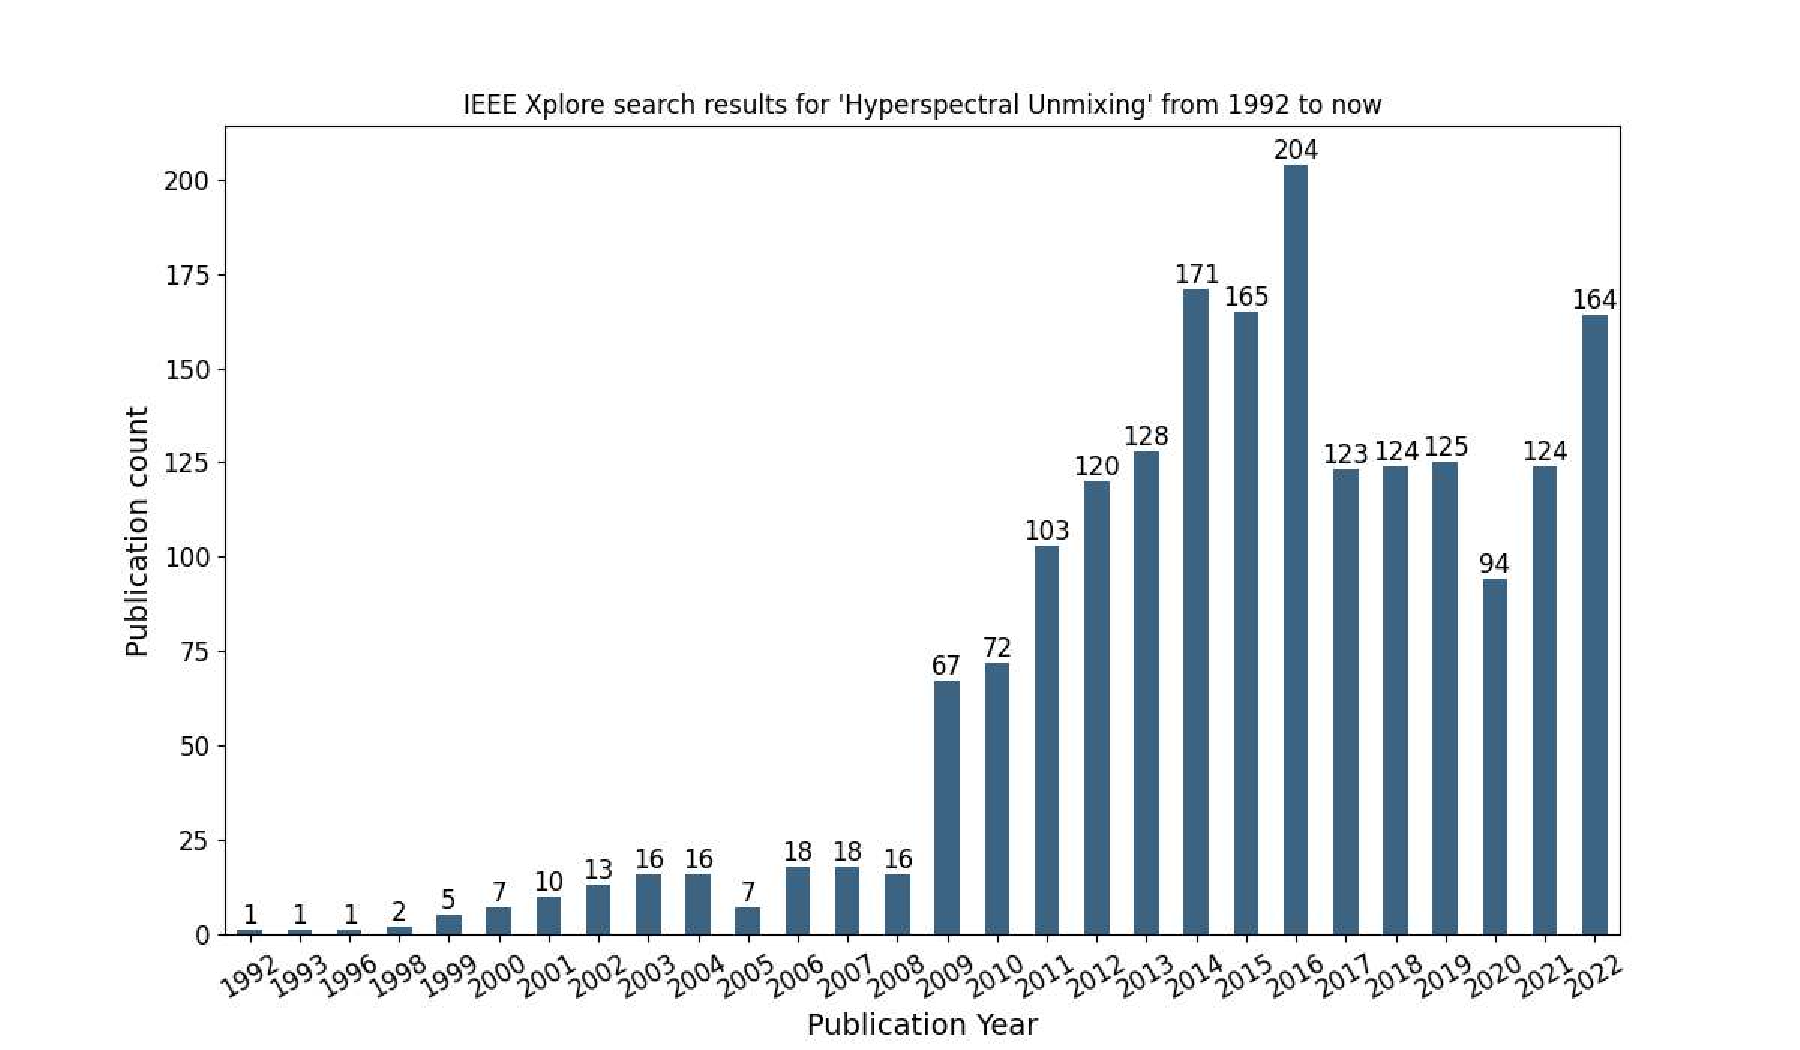
\includegraphics[width=\linewidth]{fichiers_latex/Chap4/figs/HU_results_IEEE-bigger.pdf}
    \caption{Publications over time based on IEEE Xplore keyword search tool using ``Hyperspectral Unmixing" as input.}
    \label{fig:publications}
\end{figure}

%At the time where hyperspectral unmixing gained popularity, the main scientific programming language was MATLAB as illustrated in figure \ref{fig: matlab}. However, in recent years, interest in Python rose steadily while MATLAB declined. This can be partly explained by the rise of open science whereby open sourcing scientific code became popular. Our point is that nowadays releasing an open source unmixing package in Python is more sensible than in MATLAB, even though this may require translating existing unmixing MATLAB code into Python.

During the period when hyperspectral unmixing gained popularity, the primary scientific programming language of choice was MATLAB, as depicted in figure \ref{fig:matlab}. 
However, in recent times, there has been a steady increase in interest and adoption of Python, while MATLAB's popularity has waned. 
This shift can be attributed, in part, to the growing trend of open science, where open-sourcing scientific code has become widely embraced. 
Consequently, the present scenario suggests that developing and releasing an open-source unmixing package in Python is more advantageous than doing so in MATLAB, even though it may involve the translation of existing unmixing code from MATLAB to Python.

\begin{figure}[h]
    \centering
    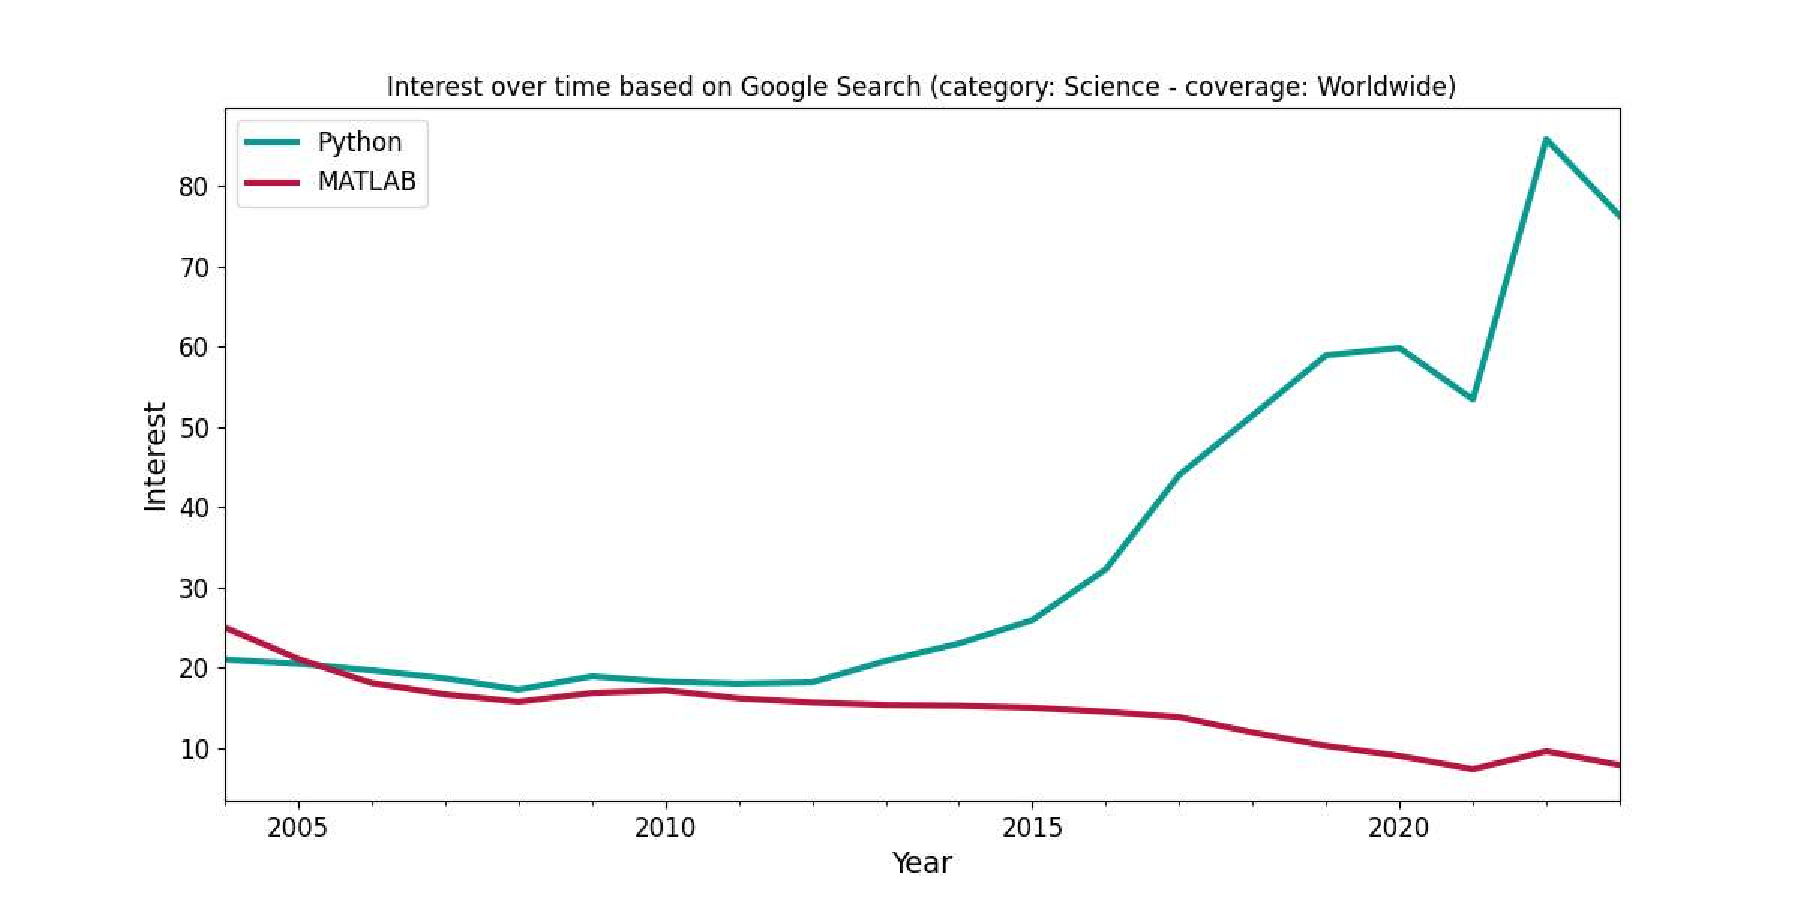
\includegraphics[width=\linewidth]{fichiers_latex/Chap4/figs/PythonVSMATLAB-bigger.pdf}
    \caption{Worldwide interest in scientific programming languages over time according to Google Trends in the ``Science" category.}
    \label{fig:matlab}
\end{figure}

\subsection{Existing overview publications and unmixing packages}

An early survey on hyperspectral unmixing was given in \cite{keshava_spectral_2002}, which discusses basic geometrical and statistical methods. In \cite{bioucas-dias_hyperspectral_2012}, linear model-based unmixing techniques were divided into three categories: geometrical, statistical, and sparse regression-based approaches. A Matlab toolbox is available at\footnote{\href{https://openremotesensing.net/}{https://openremotesensing.net/}}.  However, the toolbox is incomplete, and some methods, such as dependent component analysis (DECA), are missing. In recent years, deep learning and neural networks have become state-of-the-art for many tasks in machine learning and image processing. Consequently, many unmixing approaches were proposed based on shallow and deep neural networks. A comparison of autoencoder-based networks was drawn in \cite{palsson_blind_2022}. The authors discussed autoencoder-based architectures divided into five categories, i.e.,  Sparse Nonnegative Autoencoders,  Variational Autoencoders, Adversarial Autoencoders, Denoising Autoencoders, and Convolutional Autoencoders. They further discuss the choice of different modules, such as different activation functions or loss functions, and they compared shallow networks to deep ones. They also provide a TensorFlow-based Python package that is available on GitHub. However, the package is limited to blind unmixing approaches based on autoencoders. It does not discuss or compare the supervised, semi-supervised, and more conventional blind unmixing methods. 

In \cite{chen_integration_2023}, some model-based and neural network-based unmixing approaches were explained but without experimental comparisons. A list of resources for the approaches was given. 


%In \cite{SPM_rev}, 

A survey on endmember variability in Spectral Mixture Analysis (SMA) was given in \cite{somers_endmember_2011}. In \cite{zare_endmember_2013}, an overview of unmixing methods that address endmember variability was given. A comprehensive overview of the unmixing methods that address spectral variability was recently provided in \cite{borsoi_spectral_2021}, and a list of Matlab codes was also given. In \cite{plaza_recent_2011}, an overview of endmember extraction approaches was given. Review papers on hyperspectral remote sensing data analysis briefly discussed the unmixing methods \cite{bioucas-dias_hyperspectral_2013, ghamisi_advances_2017}. In \cite{heylen_review_2014}, a survey of nonlinear unmixing methods is given.


%\subsection{Existing Unmixing Tools and Packages}
%openremotesensing
There are other open-source tools such as HyperMix \cite{jimenez_hypermix_2015}, Spectral Python (SPy) \footnote{\href{https://www.spectralpython.net/}{https://www.spectralpython.net/}}, Spectral Library Tool \footnote{\href{https://spectral-libraries.readthedocs.io/en/latest/}{https://spectral-libraries.readthedocs.io/en/latest/}}, PySptools\footnote{\href{https://pypi.org/project/pysptools/}{https://pypi.org/project/pysptools/}}, that include basic algorithms for estimation of the number of endmembers, endmember extraction, abundance estimation, and some library tools, and library-based methods. Thus, there is a need for a comprehensive package that covers the methodologies across different unmixing categories and contains state-of-the-art image processing and machine learning techniques. 

\subsection{Contributions}

This chapter covers the following: 
\begin{itemize}
     \item  Categorizing the unmixing approaches depending on the prior knowledge available about endmembers.  Linear unmixing can be divided into three main categories:  supervised, semi-supervised (library-based), and unsupervised (blind) unmixing. 
     \item Comparing the unmixing methods in terms of prior knowledge of the endmembers and draw conclusions that can help researchers to select an appropriate unmixing method to tackle real-world challenges. We compare conventional and deep learning-based unmixing approaches in those categories for three simulated and two real-world datasets.  For the simulated datasets, we consider three scenarios: a simple, pure pixel dataset, a dataset with spectral variations, and a challenging dataset with no pure pixel. Such comparisons provide insight to researchers into which category to use for their application. Additionally, the comparisons reveal the drawbacks of the categories, which motivate the developers to investigate new ideas to address them.
     \item Providing an open-source HyperSpectral Unmixing Python Package (HySUPP). HySUPP is the first open-source python-based hyperspectral unmixing package to include supervised, semi-supervised, and blind unmixing methods.  The package will benefit the geoscience and remote sensing community, including researchers, developers, lecturers, and students. The package installation is straightforward since HySUPP relies on a few dependencies. In addition, all the methods can be run using a single command line instruction. 
 \end{itemize}

\section{HySUPP Toolbox}

HySUPP exhibits a list of highly desirable properties summarized as follows: i) completeness, ii) reproducibility, iii) extensibility and iv) homogeneity. It implements common best practices and enables simple benchmarking of unmixing techniques thanks to user-friendly command line instructions.

\subsection{Features}

\paragraph{Completeness}

As a practitioner, the ability to explore and experiment with different unmixing techniques is crucial since no single approach can consistently outperform others in all unmixing scenarios. 
Thus, ensuring the completeness of our toolbox becomes essential. 
Our toolbox is designed to cover all three types of unmixing - supervised, semi-supervised, and unsupervised - while striving to be as representative as possible of the various unmixing approaches, although aiming for exhaustive inclusion would be impractical. 
Currently, HySUPP provides access to a diverse set of 20 different unmixing methods, including 6 supervised, 6 semi-supervised, and 8 unsupervised techniques.

\paragraph{Reproducibility}

Ensuring experimental reproducibility is crucial when exploring various unmixing techniques, as it guarantees the robustness of the conclusions drawn by users. 
In line with this principle, our toolbox offers the ability to seed experiments, facilitating reproducibility through repeatable noise generation.
Additionally, HySUPP automatically saves estimates outputs, providing users with a convenient way to review and compare results, thus enhancing the reliability of their research findings.

\paragraph{Extensibility}

HySUPP's architecture is designed to support the effortless integration of new methods, providing a platform for future advancements in hyperspectral unmixing. 
Leveraging configuration files, we empower researchers to conduct experiments with ease and flexibility, enabling them to effortlessly incorporate their own models into the toolbox.

\paragraph{Homogeneity}

The uniformity of HySUPP's codebase ensures consistency across different components, enhancing its overall usability and reliability. 
More specifically, we use common methods for models and common attributes for datasets.


\paragraph{Best practices}

We offer a straightforward yet potent method to monitor the objective function of each approach using Python's \texttt{tqdm} library. 
Furthermore, our pipeline incorporates precise endmember auto-alignment through the utilization of the \texttt{munkres} algorithm, provided ground truth abundance maps are accessible. 
This enhancement ensures the accurate computation of unmixing performance. 
By establishing these best practices, we streamline the implementation process and foster a collaborative environment where researchers can easily build upon existing work and share their contributions effectively.



\paragraph{Benchmarking}

Owing to its rich set of features, HySUPP enables users to easily benchmark all implemented methods on their dataset of choice. 
Our toolbox currently provides 3 synthetic datasets corresponding to different unmixing scenarios.
Moreover, we incorporate 4 distinct metrics to thoroughly evaluate unmixing accuracy across methods.
Finally, leveraging \texttt{mlxp}~\cite{arbel_mlxp_2023} results query tool, we empower users to analyze and visualize their results in an appealing and informative manner.

\subsection{Example}

The following command line instruction provides an example on how to run a semi-supervised unmixing technique, \texttt{SUnCNN}~\cite{rasti_suncnn_2022}, on the \texttt{DC1} dataset using an optional custom value for the signal-to-noise ratio (SNR):

\texttt{\$ python unmixing.py mode=semi data=DC1 model=SUnCNN noise.SNR=30}

Table \ref{tab:toolbox_desc} lists unmixing methods included in HySUPP with their corresponding dependencies. We highlighted our main contributions and the link to the original implementations.
\begin{table}[h]
    \centering
    \caption{The list of unmixing methods included in HySUPP with their corresponding dependencies. We highlighted our main contributions and the link to the original implementations. }
    \resizebox{\textwidth}{!}{
    \begin{tabular}{c|c c c c c}
    \toprule
         Method & Source & Python & Dependencies & GPU & Contributions \\
    \midrule
          FCLSU~\cite{heinz_fully_2001} & \href{https://pysptools.sourceforge.io/_modules/pysptools/abundance_maps/amaps.html#FCLS}{pysptools} & \checkmark & \texttt{numpy}, \texttt{cvxopt} & & Refactor into a \texttt{SupervisedUnmixingModel} sub-class\\
          SiVM~\cite{heylen_fully_2011} & \href{https://github.com/BehnoodRasti/MiSiCNet/blob/main/UtilityMine.py}{github}& \checkmark & \texttt{numpy} & & Refactor into a \texttt{BaseExtractor} sub-class \\
          SISAL~\cite{bioucas-dias_variable_2009} & \href{https://github.com/etienne-monier/lib-unmixing}{github} & \checkmark & \texttt{numpy} & & Refactor into a \texttt{BaseExtractor} sub-class \\
          UnDIP~\cite{rasti_undip_2021} & \href{https://github.com/BehnoodRasti/UnDIP}{github} & \checkmark & \texttt{torch} & \checkmark & Refactor separate scripts into a single model\\
          VCA~\cite{nascimento_vertex_2003} & \href{https://github.com/Laadr/VCA}{github} & \checkmark & \texttt{numpy} & & Replace \texttt{scipy} dependency by \texttt{numpy}. Add random seed\\
    \midrule
          CLSUnSAL~\cite{iordache_collaborative_2014}& \href{https://github.com/etienne-monier/lib-unmixing}{github}& \checkmark & \texttt{numpy} & & Implementation based on SUnSAL\\
          MUA\_SLIC~\cite{borsoi_fast_2019}& \href{https://github.com/ricardoborsoi/MUA\_SparseUnmixing}{github} & \checkmark & \texttt{numpy}, \texttt{skimage} & & MATLAB code translation using \texttt{skimage}'s SLIC\\
          S$^2$WSU~\cite{zhang_hyperspectral_2018} & \href{https://github.com/ricardoborsoi/MUA\_SparseUnmixing}{github} & \checkmark & \texttt{numpy}, \texttt{scipy} & & MATLAB code translation\\
          SUnAA~\cite{rasti_sunaa_2023} & \href{https://github.com/inria-thoth/SUnAA}{github} & \checkmark & \texttt{numpy}, \texttt{spams} & & Refactor to match \texttt{SemiUnmixingModel} sub-class\\
          SUnCNN~\cite{rasti_suncnn_2022} & \href{https://github.com/BehnoodRasti/SUnCNN}{github} & \checkmark & \texttt{torch} & \checkmark & Refactor separate scripts into a single model \\
          SUnSAL~\cite{bioucas-dias_alternating_2010} & \href{https://github.com/etienne-monier/lib-unmixing}{github} & \checkmark & \texttt{numpy} & & Refactor into \texttt{SemiUnmixingModel} sub-class \\
    \midrule
          ADMMNet~\cite{zhou_admm-based_2021} & - & \checkmark & \texttt{torch} & \checkmark & Implemented from scratch\\
          BayesianSMA~\cite{dobigeon_joint_2009} & \href{https://ndobigeon.github.io/applications/app_hyper_SMA.html}{webpage} & \texttt{matlab.engine} & \texttt{numpy} & & Python wrapper around existing MATLAB code\\
          CNNAEU~\cite{palsson_convolutional_2020} & \href{https://github.com/burknipalsson/hu\_autoencoders}{github}& \checkmark & \texttt{torch} & \checkmark & Convert existing \texttt{keras} implementation into \texttt{torch}\\
          EDAA~\cite{zouaoui_entropic_2023} & \href{https://github.com/inria-thoth/EDAA}{github} & \checkmark & \texttt{torch} & \checkmark & Refactor to match \texttt{BlindUnmixingModel} sub-class\\
          MiSiCNet~\cite{rasti_misicnet_2022} & \href{https://github.com/BehnoodRasti/MiSiCNet}{github}& \checkmark & \texttt{torch} & \checkmark & Refactor separate scripts into a single model \\
          MSNet~\cite{yu_multi-stage_2022} & \href{https://github.com/yuyang95/JAG-MSNet}{github}& \checkmark & \texttt{torch} & \checkmark & Refactor to match \texttt{BlindUnmixingModel} sub-class \\
          NMFQMV~\cite{zhuang_regularization_2019} & \href{https://github.com/LinaZhuang/NMF-QMV\_demo}{github}& \texttt{matlab.engine} & \texttt{numpy} & & Python wrapper around existing MATLAB code \\
          PGMSU~\cite{shi_probabilistic_2021} & \href{https://github.com/shuaikaishi/PGMSU}{github}& \checkmark & \texttt{torch} & \checkmark & Refactor to match \texttt{BlindUnmixingModel} sub-class\\
    \bottomrule
    \end{tabular}
    }
    \label{tab:toolbox_desc}
\end{table}

\section{Experiments}

We use three simulated and one real datasets. The simulated datasets were designed according to different mixing scenarios briefly explained in Table \ref{tab:data_description}. We avoid using the widely used benchmark datasets such as Samson and Jasper since their abundances are generated synthetically. For real-world experiments, we use the Cuprite dataset, a well-studied site with geological reference maps. The simulated experiments were carried out for 30 dB SNR. The tuning parameters were fine-tuned for the methods up to some levels. We should note that some methods have several parameters to be tuned; therefore, searching for the optimum is cumbersome. All the results are averaged over 10 experiments, and the standard deviations are shown by error bars. In experiments, we compare 20 unmixing methods from different categories as follows. For supervised methods, we used three endmember extraction/estimation techniques, i.e., VCA, SiVM, and SISAL with FCLSU and UnDIP. All six combinations of them were considered. For blind unmixing, we use PGMSU, MSNET, CNNAEU, ADMMNet, BayesianSMA, NMFQMV, MiSiCNet, and EDAA. For sparse unmixing, we used SUnSAL, CLSUnSAL, MUA\_SLIC, S$^2$WSU, SUnCNN, and SUnAA. The codes for all those methods were provided in  HySUPP for reproducibility.  

For the quantitative evaluation, we use the SRE in dB for estimated abundances given by
\begin{equation}
    \text{SRE}(\X, \hat{\X})=20\log_{10}\frac{\|{\X}\|_F}{\|{\X}-\hat{\X}\|_F}.
\end{equation}

\subsection{Data description}

\subsubsection{Synthetic Datasets with Spatial Structure}

We simulated three data cubes (DC1, DC2, and DC3). DC1 was simulated using a linear mixing model with 5 endmembers selected from the USGS library and 75$\times$75 pixels. The abundance maps are composed of five rows of square regions uniformly distributed over the spatial dimension. This dataset contains pure pixels for all endmembers. DC2 has 100$\times$100 pixels and was simulated using a linear mixing model with 9 endmembers. The abundance maps were sampled
from a Dirichlet distribution centered at a Gaussian
random field to have piece-wise smooth maps with steep transitions. Therefore, DC2 contains spectral variations. For DC1 and DC2, an endmember library $\D \in \mathbb{R}^{188\times 240}$, composed of 240 spectral signatures were selected from the USGS library with a minimum pair-spectra angle of 4.44\textdegree. DC3 was simulated with no pure pixels, and it has two mixed pixels on the facet of the data simplex. DC3 is composed of  105$\times$105 pixels using the linear combination of six endmembers. For DC3, we use a library $\D \in \mathbb{R}^{188\times 498}$ composed of 498 spectral pixels from the USGS library. Note that we remove the water absorption and noisy bands, and therefore, the final pixels are of dimension $p=188$.

\subsubsection{Cuprite Dataset}
The Cuprite dataset used in this paper contains 250$\times$ 191 pixels. Cuprite is a well-studied mineral site, and the dominant minerals are demonstrated using a geological ground reference therefore, the estimated abundance maps by different techniques can be compared visually.
We use the same library as explained for DC3. 


\begin{table}[h]
    \centering
    \caption{Specifications of the synthetic datasets used in the experiments.}
    \resizebox{\textwidth}{!}{
    \begin{tabular}{c|c c c c }
    \toprule
         & \# endmembers ($r$) & \# atoms in ${\bf D}$ ($m$) & \# pixels ($n$) & Main features \\
    \midrule
        DC1 & 5 & 240 & 5625 (75 $\times$ 75)  & Pure pixels\\
        DC2 & 9 & 240 & 10000 (100 $\times$ 100)  & Pure pixels, Spectral variability\\
        DC3 & 6 & 498 & 11025 (105 $\times$ 105)  & No pure pixels, 2 points on the data simplex facets\\
        
    \bottomrule
    \end{tabular}
    }
    \label{tab:data_description}
\end{table}

\subsection{Synthetic datasets}

Figure \ref{fig:DC1_30dB_SRE} demonstrates the unmixing results in terms of abundance SRE in DB for different techniques applied to DC1, DC2, and DC3. The outcomes of the results can be summarized as follows: 
\begin{itemize}
    \item For the pure pixel scenario, supervised techniques perform very well (Fig. \ref{fig:DC1_30dB_SRE}, DC1). Overall, they perform better than the semisupervised and blind techniques. This confirms the importance of geometrical information for endmember extraction/ estimation techniques when there are pure pixels in the dataset. This is further confirmed in blind methods where MiSiCNet and NMFQMV, which exploit geometrical information, outperform the other blind techniques and provide competitive results compared to supervised ones. Sparse techniques show moderate results except SUnAA, which outperforms all the other techniques. The results confirm that the sparse unmixing techniques are not suitable when there are pure pixels for the endmembers in the dataset. We should mention that SUnAA does not match the characteristics of conventional sparse techniques. Even though SUnAA relies on a library, it uses a nonconvex optimization to estimate endmembers. 
    \item On the other hand, for DC2, which contains spectral variations, as can be seen from Fig. \ref{fig:DC1_30dB_SRE}, sparse unmixing techniques outperform the supervised and blind techniques. The results confirm that sparse unmixing techniques are more suitable for capturing the spectral variability. SUnAA outperforms the other technique. Note that SUnAA is a parameter-free technique. Supervised techniques outperform blind techniques due to the presence of pure pixels. 
    \item In the case of no pure pixel scenario (Fig. \ref{fig:DC1_30dB_SRE}, DC3), blind unmixing techniques that exploit geometrical information outperform the other techniques. Sparse unmixing provides very poor results. Although SUnAA considerably significantly outperforms the performance of sparse unmixing techniques, it is very far from the best performance which is obtained by MiSiCNet. Among supervised techniques, SISAL (+ FCLSU/UnDIP) shows competitive results because it uses geometrical information to estimate the endmembers.  
\end{itemize}


\begin{figure}[h]
   \centering
   \begin{tabular}{c} 
   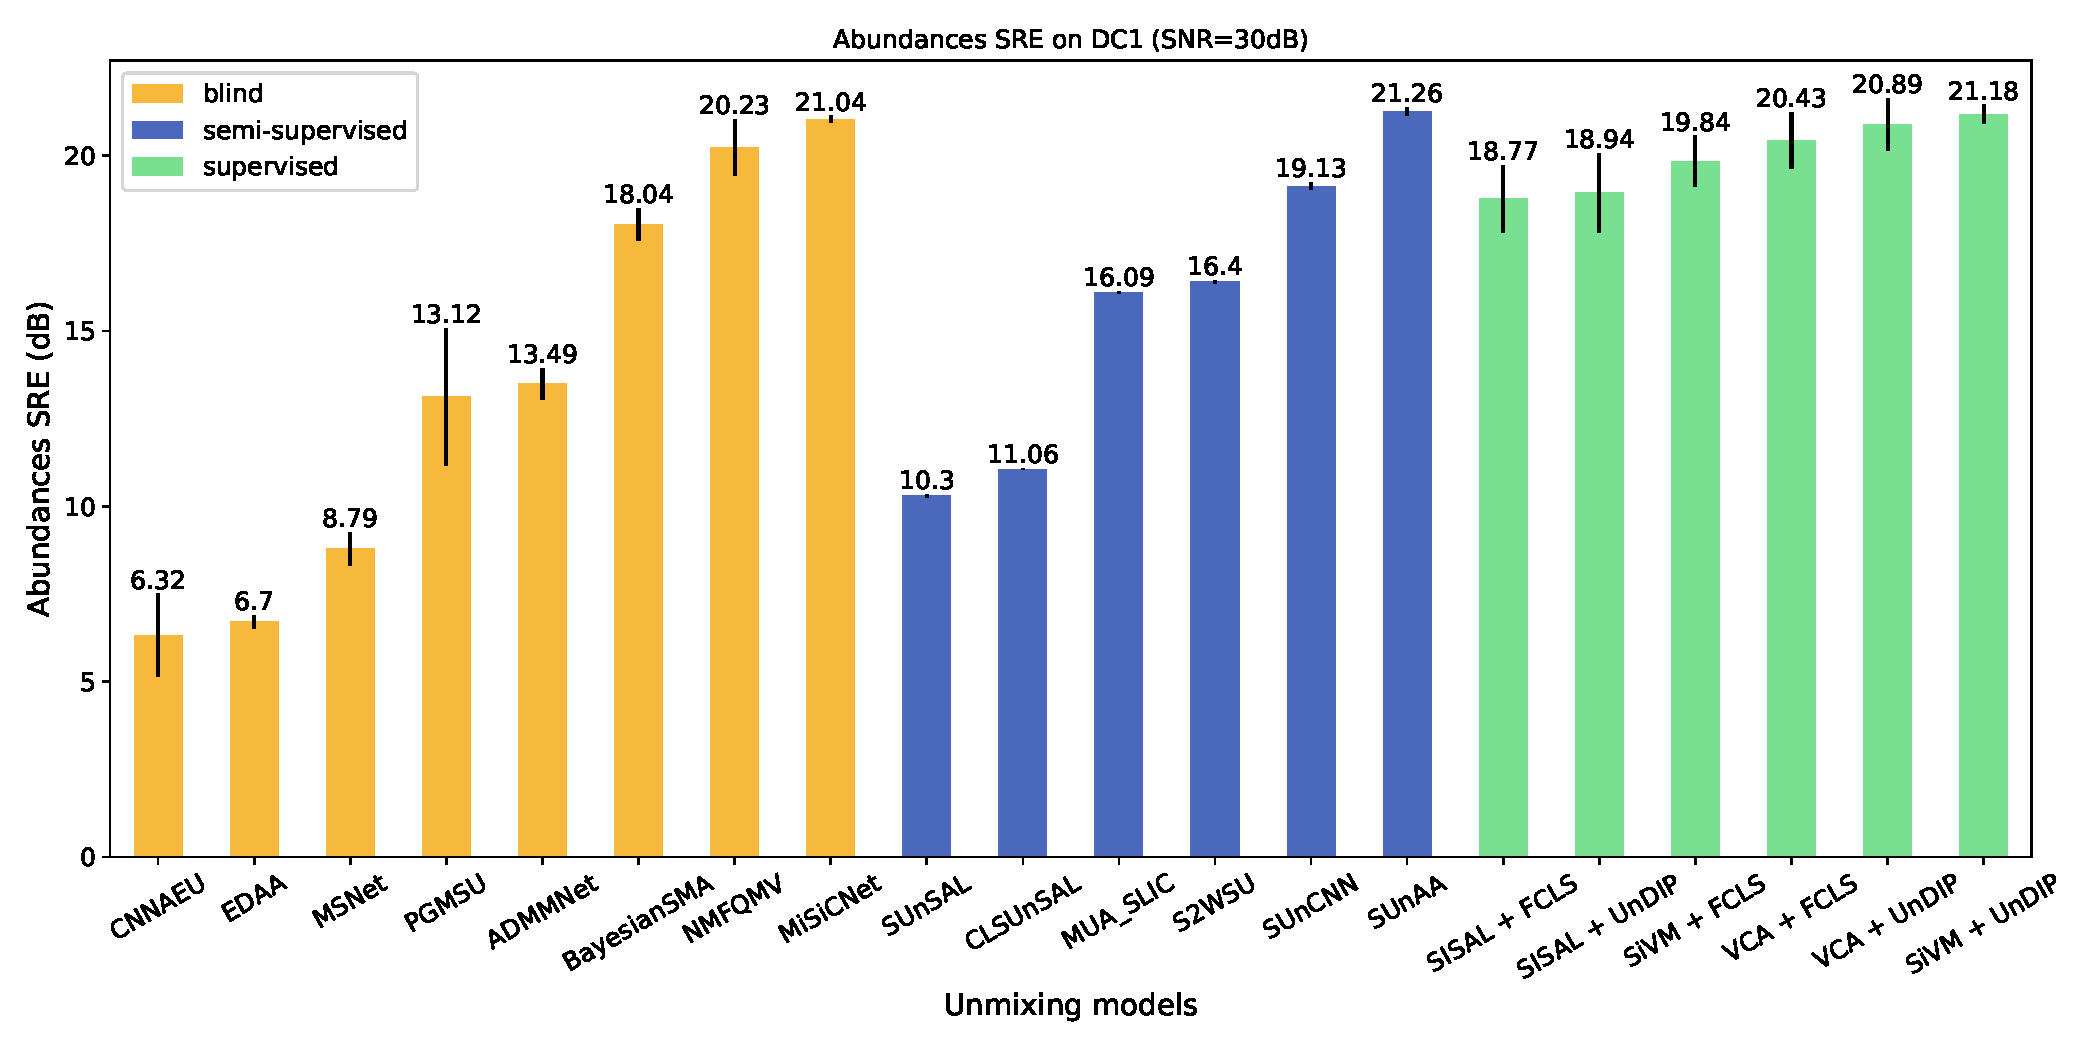
\includegraphics[width=.8\textwidth]{fichiers_latex/Chap4/figs/DC1_30.pdf}\\   
   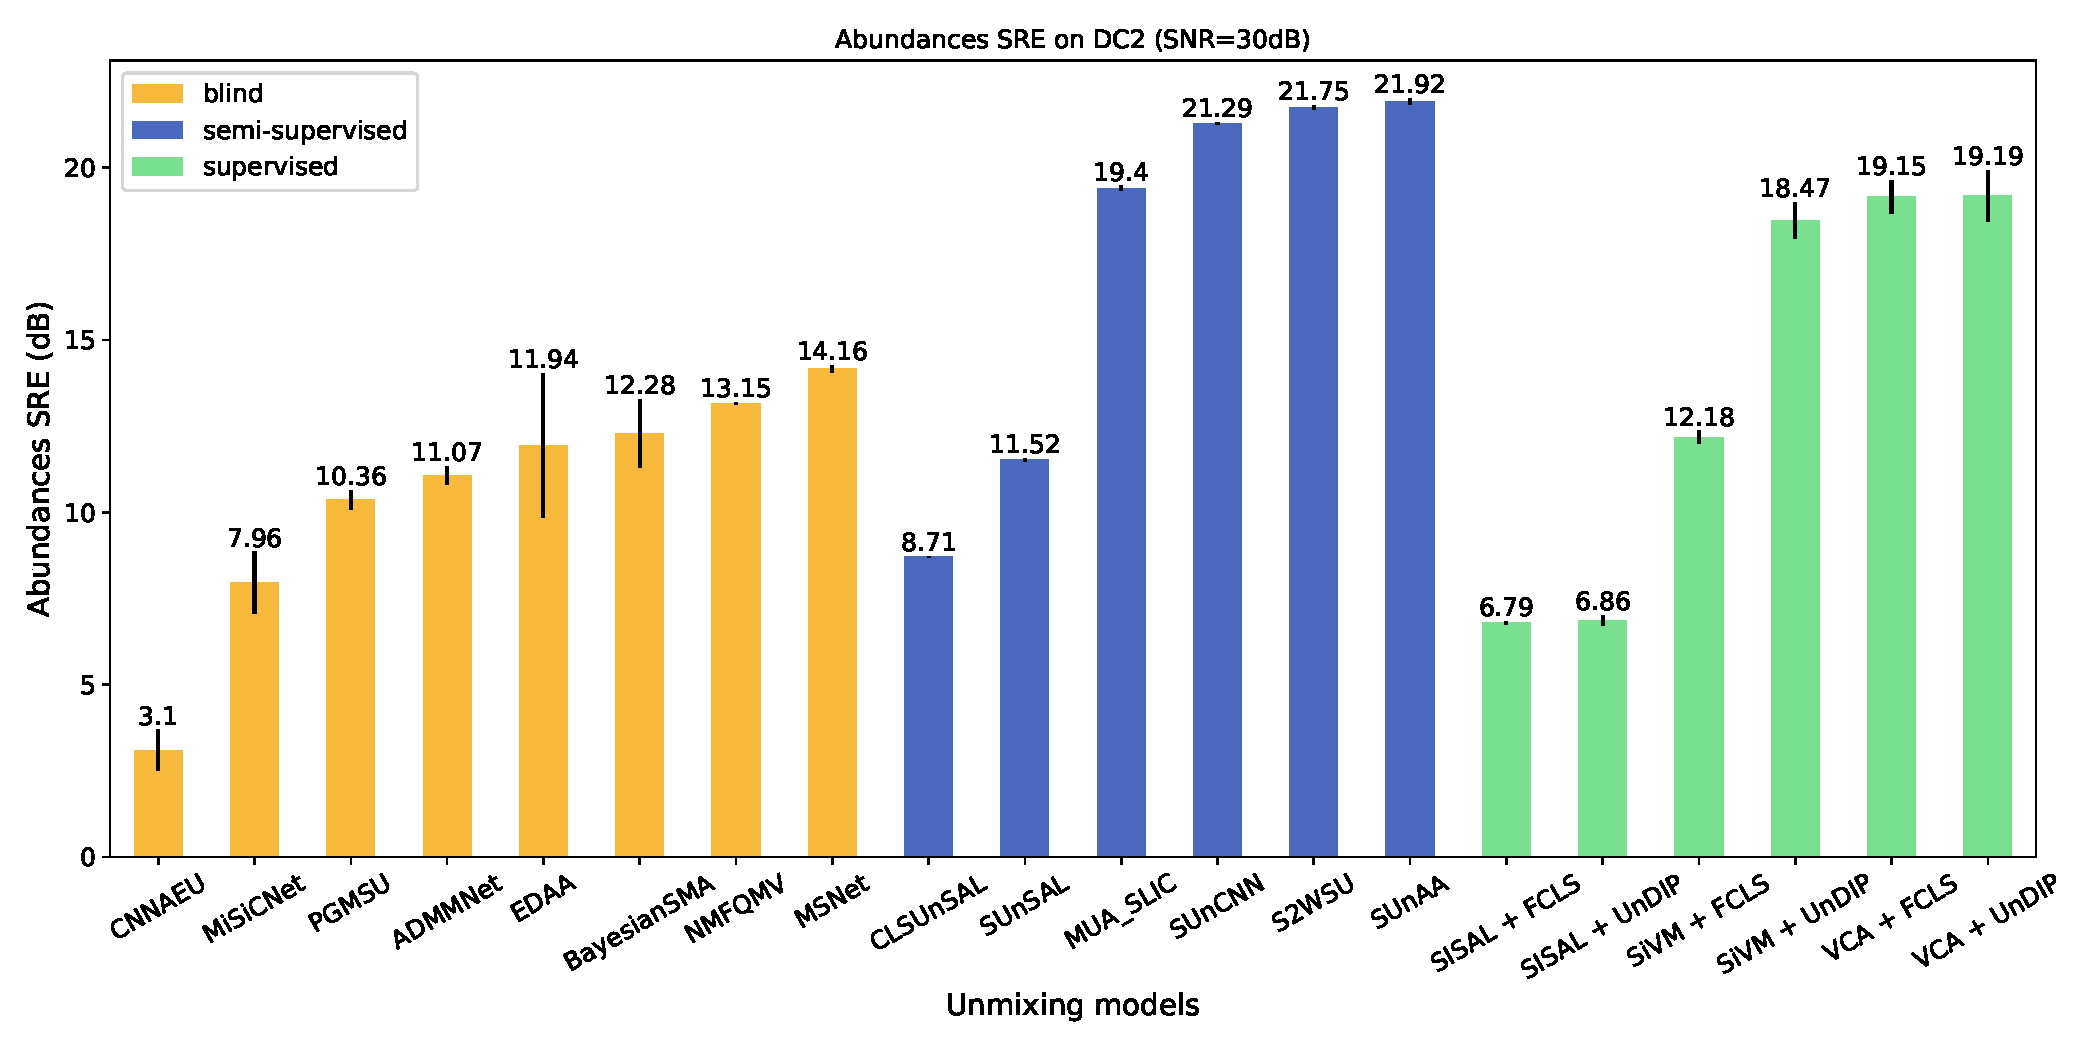
\includegraphics[width=.8\textwidth]{fichiers_latex/Chap4/figs/DC2_30.pdf}
\\ 
   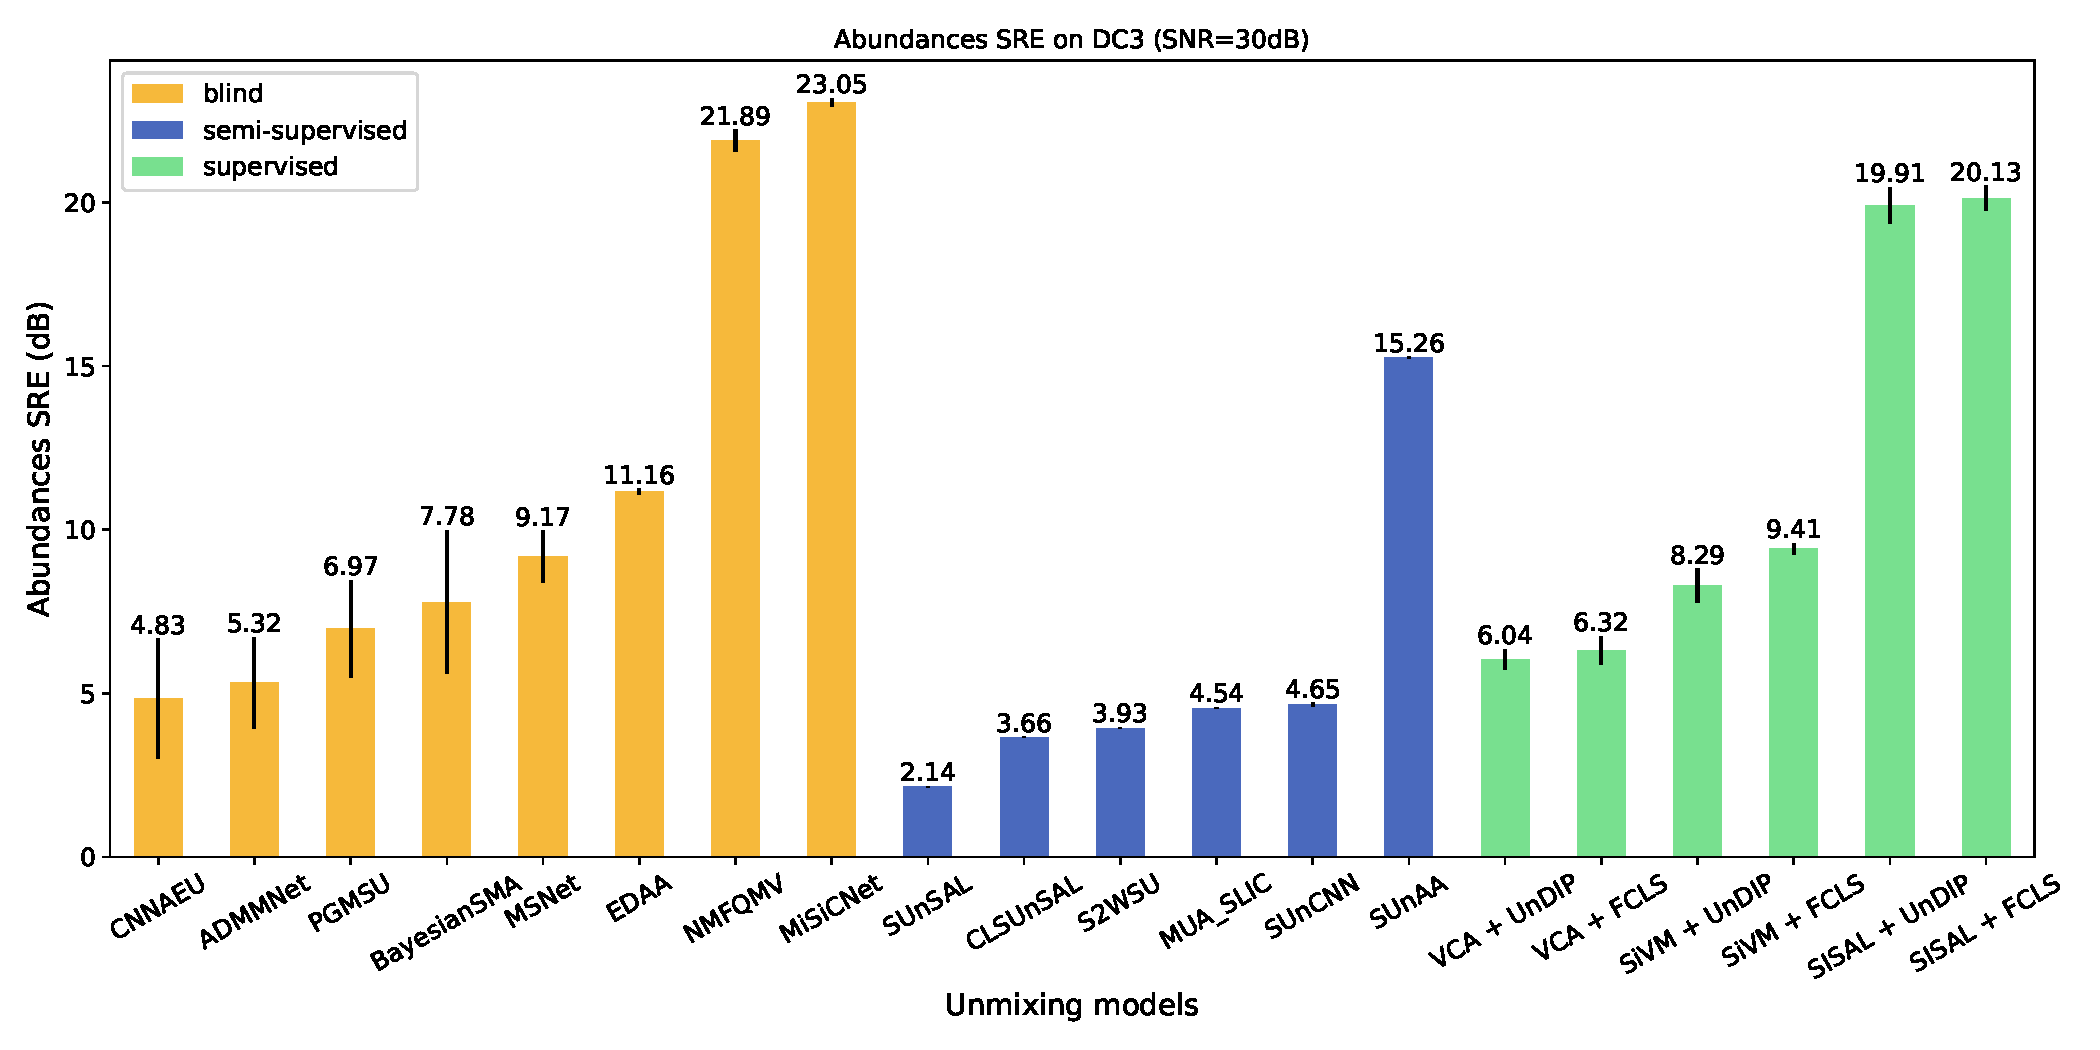
\includegraphics[width=.8\textwidth]{fichiers_latex/Chap4/figs/DC3_30.pdf}
 \end{tabular} 
   \caption{Comparing abundance SRE ($\uparrow$) in dB using different unmixing techniques applied to (from top to bottom) synthetic DC1, DC2, and DC3.}
   \label{fig:DC1_30dB_SRE}
\end{figure}

\subsection{Real data}

We selected three methods per category to conduct unmixing on the Cuprite dataset. 
Blind unmixing: MiSiCNet, MSNet and NMFQMV. 
Semi-supervised: SUnAA, MUA\_SLIC, S$^2$WSU.
Supervised: UnDIP combined with SISAL, SiVM and VCA.
We describe the hyperparameters that were fine-tuned for the following techniques.
The hyperparameters set as default are omitted.
\begin{itemize}
    \item MiSiCNet: $\lambda=100$, \texttt{projection=True}.
    \item MSNet: $\alpha=0.1$, $\beta=0.1$.
    \item MUA\_SLIC: $\beta=30$, $\lambda_1=0.001$, $\lambda_2=0.001$, $\text{slic\_size}=200$.
    \item S$^2$WSU: $\lambda=0.001$.
    \item SISAL: $\tau=1\text{e-}6$.
\end{itemize}

Fig. \ref{Real dataset} (b) visually compares the estimated abundances for three dominant minerals, i.e., Chalcedony, Alunite, and Kaolinite. The comparison with the geological reference map Fig. \ref{Real dataset} (a) reveals that the estimated abundances obtained by semisupervised methods show more resemblance to the reference map for all three minerals. SUnAA visually outperforms the other techniques, particularly in the case of Chalcedony. The blind unmixing methods can better estimate Chalcedony compared to MUA\_SLIC and S$^2$WSU. This could be attributed to the mismatch of the endmember with the library's endmembers for this mineral. It is worth mentioning that SUnAA does not entirely rely on the library, and it estimates the endmember. Therefore, it can compensate for such a mismatch. More importantly, SUnAA is a parameter-free technique. We should note that selecting optimum parameters for the unmixing techniques is not a trivial task in real-world applications since the abundance RMSE cannot be computed.   

\begin{figure}[h]
\centering
  \begin{tabular}{cc}
%   \includegraphics[width=.15\textwidth]{Cuprite_RGB.png}&
   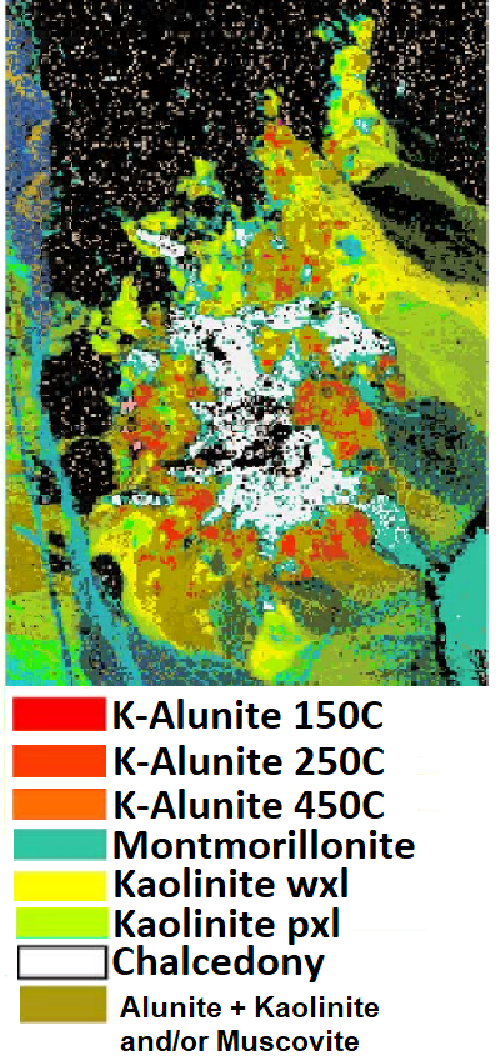
\includegraphics[width=.14\textwidth]{fichiers_latex/Chap4/figs/Cuprite_GT_image3.pdf}&   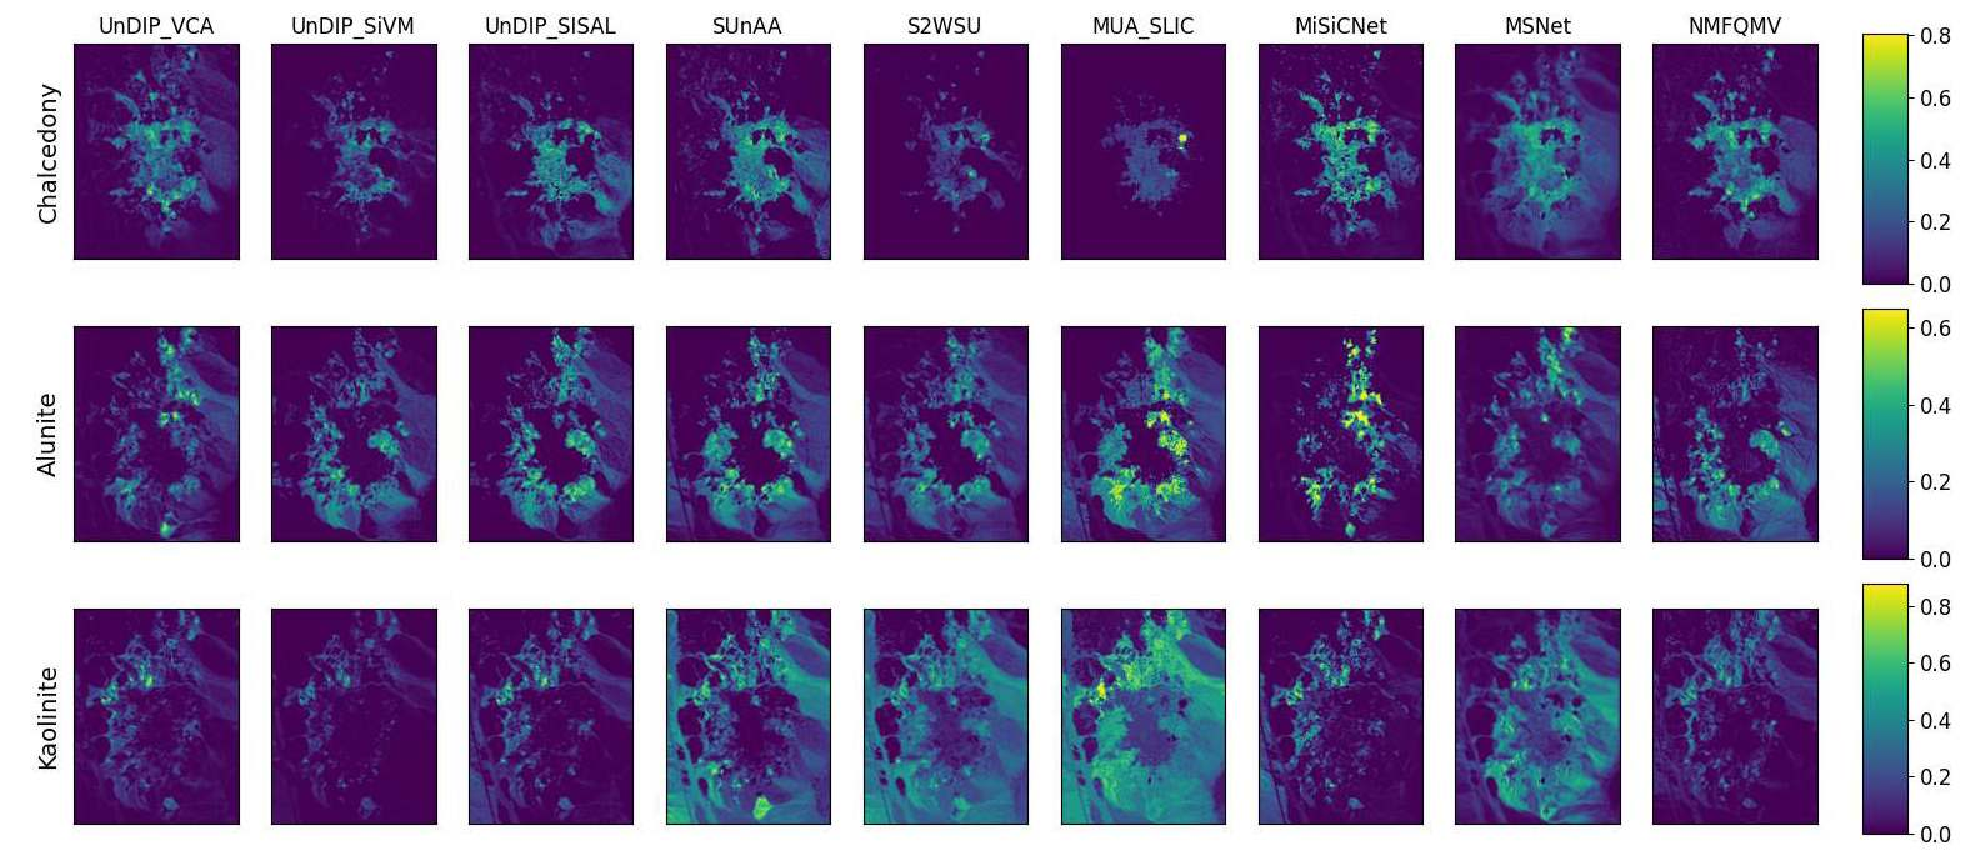
\includegraphics[width=.75\textwidth]{fichiers_latex/Chap4/figs/Cuprite2.pdf}\\
 (a) Geological Ref. Map & (b) Estimate abundances
  \end{tabular}
  \caption{Estimate abundances obtained by applying different unmixing techniques to Cuprite compared with the geological reference map.}
\label{Real dataset}
\end{figure}

\section{Discussion and Conclusion}

Assuming that we have captured a spectral dataset and now have an unmixing problem in hand, we need to estimate the abundances of materials. The main question is which method to choose and which group of methods to select to tackle the problem. Indeed, the first step is to evaluate our problem and see if the linear mixing model or its variations are suitable for our problem. This decision needs prior knowledge of the physics of the problem. For instance, if you are dealing with intimate mixtures or close-range and microscopic scenarios, you should use nonlinear models. If you are dealing with macroscopic Earth observation problems, then linear models or their variations will be suitable. In some research, nonlinear models perform better than linear ones, however, one may pay attention to the selection of the model in a real-world application. Usually, linear models are more general. 

Here, we clarify the keys to the success of each category. The success of supervised (or sequential) unmixing lies in the confidence of the endmember measured, extracted, or estimated (pure/no pure scenario). Therefore, we should not use the supervised method if we are not confident about the endmembers. In other words, supervised methods perhaps are the best choice for endmembers with high confidence. When we have prior information on the material in the scene and a well-designed endmember library, semi-supervised unmixing could be successful. Semi-supervised are also suitable to capture the spectral variability. The success of semi-supervised unmixing lies in the quality of the endmember library. Blind unmixing methods should be selected when there is no library, no pure pixels in the data set (including highly mixed scenarios), or the confidence of the measure, selected, or estimated endmembers is low. They should be used with caution, and the estimated endmembers should always go through physical interpretation. 
